\uuid{tTH6}
\exo7id{4955}
\titre{exo7 4955}
\auteur{quercia}
\organisation{exo7}
\datecreate{2010-03-17}
\isIndication{false}
\isCorrection{true}
\chapitre{Géométrie affine euclidienne}
\sousChapitre{Géométrie affine euclidienne du plan}
\module{Géométrie}
\niveau{L2}
\difficulte{}

\contenu{
\texte{
Soit $ABC$ un triangle d'angles $\alpha,\beta,\gamma$.

On note $\rho,\rho',\rho''$ les rotations autour de $A,B,C$ d'angles
$\alpha,\beta,\gamma$, orientés suivant le dessin :
$$
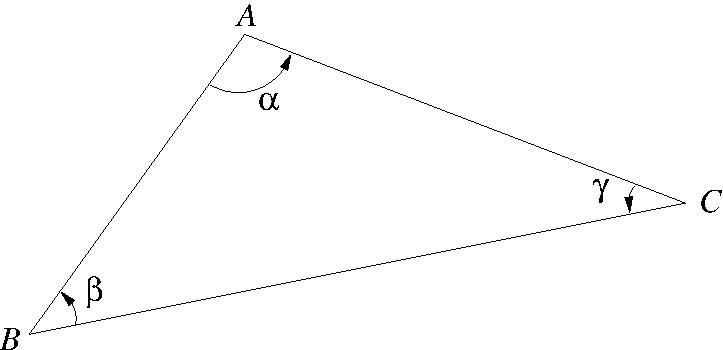
\includegraphics[height=3cm]{../images/pdf/tTH6-1.pdf}
$$

Qu'est-ce que $\rho \circ \rho' \circ \rho''$ ?
}
\reponse{
la symétrie centrale ($\alpha + \beta + \gamma = \pi$) autour de $K$, point
de contact du cercle inscrit et de $(AC)$.
}
}
